\documentclass[a4paper,12pt]{article}
 \usepackage[italian]{babel} 
\usepackage{graphicx}
\usepackage{caption}
\usepackage{geometry}
\usepackage{enumitem}
\usepackage{fancyhdr}
\usepackage{svg-extract}
\usepackage{hyperref}
\geometry{a4paper, top=1.5cm, bottom=1.5cm, left=1.5cm, right=1.5cm, }
\setlength{\parindent}{0pt} %\setlength{\parskip}{0,25cm plus1mm minus1mm}
\graphicspath{ {/Users/nicola/Documents/GitHub/lifemanager/images/Latex/} } 
\lhead{
\includegraphics[width=5cm]{logounitn.jpg}}
\rhead{
\includegraphics[width=3cm]{logolifemanager.png}}
\setlist[itemize]{leftmargin=5.5mm}




%\fancyhead[L]{
\includegraphics[width=5cm]{logounitn.jpg}}
\renewcommand{\headrulewidth}{0pt}
\raggedbottom

%-----------------------------------------TITOLO
 \title{LifeManager}
 \author{
 Corso di Ingegneria del software\\ \\Luca Boschiero, Mauro Meneghello, Nicola Turniano
 }
 \begin{document} 
 \maketitle
 \thispagestyle{fancy}
 %-----------------------------------------INFORMAZIONI STUD
\hrule
\begin{table}[!h] 
\begin{tabular}{l l l}
Gruppo T10\\
Deliverable 2\\
 \\
Mauro Meneghello & 217564 & mauro.meneghello@studenti.unitn.it \\
Luca Boschiero & 217460 & luca.boschiero@studenti.unitn.it \\
Nicola Turniano  & 271457 & nicola.turniano@studenti.unitn.it \\
\end{tabular}
\end{table}
\hrule
\vspace{1cm}

 %-----------------------------------------SVOLGIMENTO


\section*{Analisi dei componenti}
Nel seguente capitolo analizzeremo i componenti interni che costituiranno il nostro sistema, andando a definire una prima architettura al software {\scshape LifeManager}, e le relazioni tra questi componenti. 

In particolare, un componente rappresenta un’entità autonoma all’interno di un sistema o sottosistema; esso ha una o più interfacce (fornite o richieste), e gli elementi al suo interno sono nascosti ed inaccessibili eccetto che attraverso i mezzi forniti dalle sue interfacce.


Il risultato di questa analisi costituirà i vari \textit{Component Diagrams }riportati nelle figure sottostanti; inoltre per ogni singolo componente sarà descritto lo scopo e le sue interfacce.

\begin{center}
  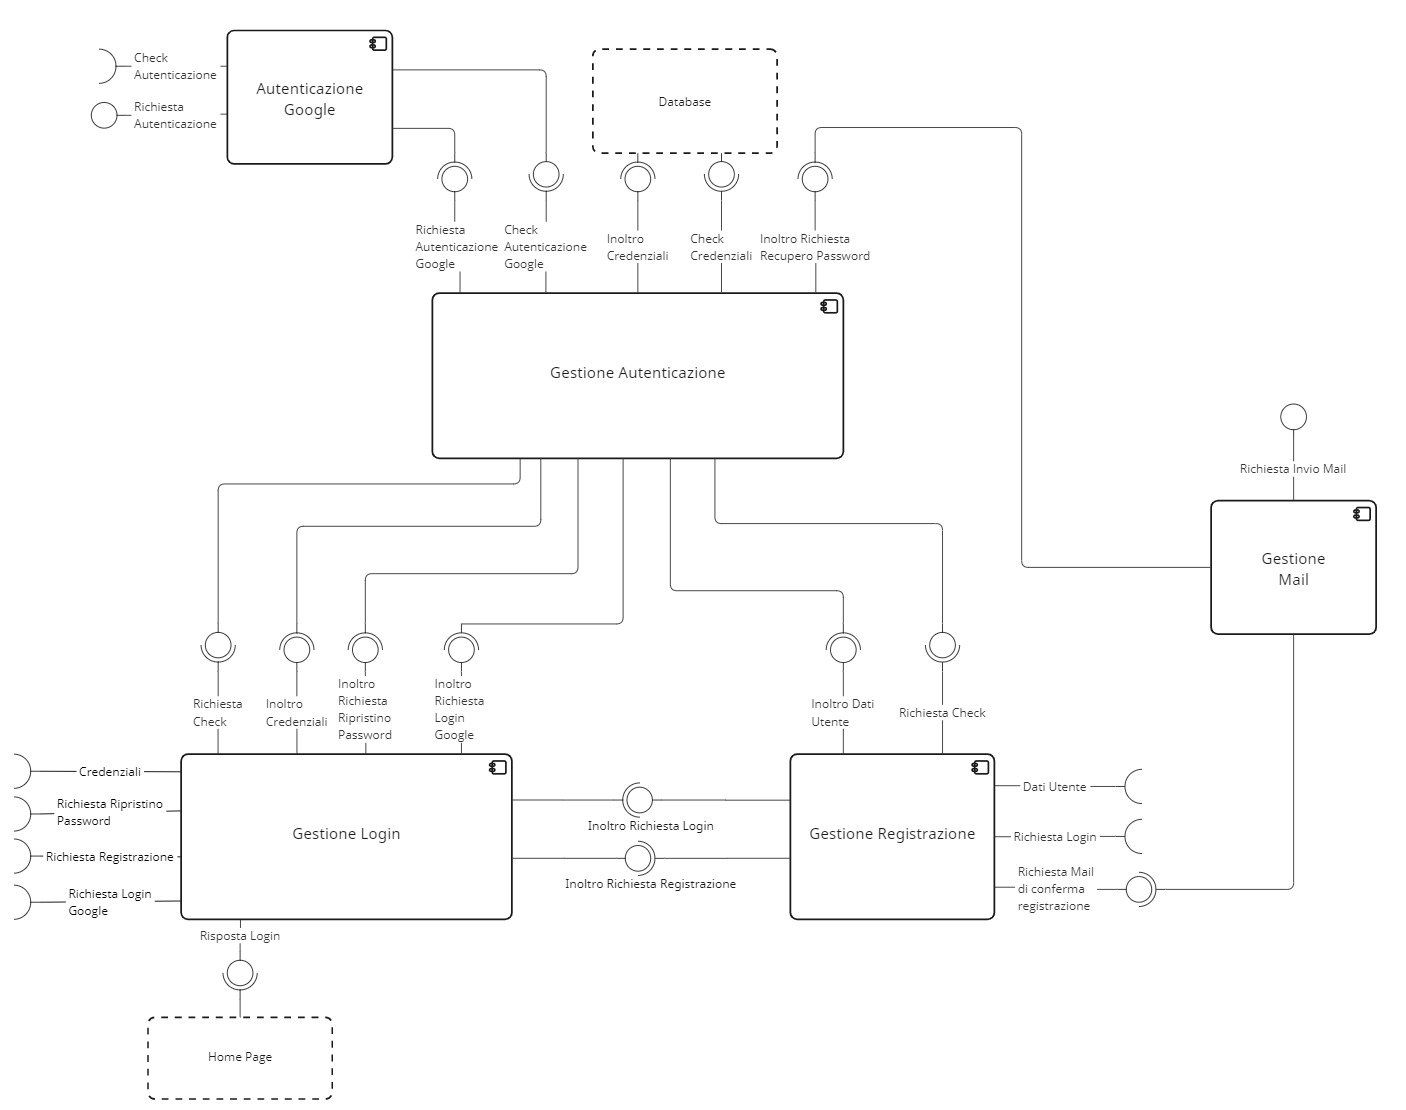
\includegraphics[width=15cm]{LoginRegistrazioneAutenticazione.jpg}
  \captionof{figure}{Component diagram Login, Registrazione, Autenticazione }
\end{center}

\subsection*{1 - Gestione Login}
\subsubsection*{Descrizione}
Questo componente permette di interfacciarsi direttamente con l’utente che desidera effettuare il login con le proprie credenziali. In particolare, verranno raccolti i dati dell’utente (credenziali) o eventuali richieste (recupero password) e inoltrati ad altri componenti interni per elaborarli.

\subsubsection*{Interfacce richieste}
\begin{itemize} \setlength\itemsep{0.01em}
\item {\sffamily Credenziali}: il componente riceve dall'utente username (o email) e password per accedere all'account.
\item {\sffamily Richiesta check}: il componente riceve dal componente 'Gestione autenticazione' l'esito del controllo della correttezza delle credenziali inserite dall'utente.
\item {\sffamily Richiesta ripristino password}: il componente riceve dall'utente la richiesta di ripristino della password.
\item {\sffamily Richiesta login Google}: il componente riceve dall'utente la richiesta di effettuare l'autenticazione con Google.
\item {\sffamily Richiesta registrazione}: il componente riceve dall'utente la richiesta di registrarsi e creare un nuovo account perchè non dispone ancora delle credenziali per effettuare il login.
\item {\sffamily Inoltro richiesta login}: il componente riceve la richiesta di effettuare il login dal componente 'Gestione registrazione'.
\end{itemize}

\subsubsection*{Interfacce fornite}
\begin{itemize} \setlength\itemsep{0.01em}
\item {\sffamily Risposta login}: il componente restituisce l'esito dell'operazione di autenticazione, se positivo permetterà la visualizzazione della home page tramite il componente 'Home Page' .
\item {\sffamily Inoltro richiesta registrazione}: il componente fornisce al componente 'Gestione registrazione' la richiesta di effettuare una nuova registrazione .
\item {\sffamily Inoltro credenziali}: il componente fornisce al componente 'Gestione autenticazione' le credenziali ricevute dall'utente per effettuarne i controlli.
\item {\sffamily Richiesta ripristino password}: il componente fornisce al componente 'Gestione autenticazione' la richiesta dell'utente di ripristinare la password.
\item {\sffamily Inoltro richiesta login Google}: il componente dornisce al componente 'Gestione autenticazione' la richiesta dell'utente di effettuare il login con Google.
\end{itemize}





\subsection*{2 - Gestione registrazione}
\subsubsection*{Descrizione}
Questo componente permette di interfacciarsi con l’utente per permettere la registrazione al sistema e la creazione di un nuovo account. I dati raccolti verranno smistati agli altri componenti che li elaboreranno.

\subsubsection*{Interfacce richieste}
\begin{itemize} \setlength\itemsep{0.01em}
\item {\sffamily Dati utente}: il componente, per permettere all'utente di registrarsi, richiede l'inserimento di nome, cognome, username, email e la password (ripetuta due volte).
\item {\sffamily Richiesta registrazione}: il componente riceve dal componente 'Gestione login' la richiesta dell'utente di effettuare la registrazione.
\item {\sffamily Richiesta check}: il componente riceve dal componente 'Gestione autenticazione' l'esito del controllo sui dati inseriti dall'utente.
\item {\sffamily Richiesta login}: il componente riceve dall'utente la richiesta di effettuare il login.
\end{itemize}

\subsubsection*{Interfacce fornite}
\begin{itemize} \setlength\itemsep{0.01em}
\item {\sffamily Richiesta mail conferma registrazione}: il componente fornisce al componente 'Gestione mail' la richiesta di inviare una mail all'utente per confermare l'avvenuta registrazione.
\item {\sffamily Inoltro richiesta login}: il componente fornisce al componente 'Gestione login' la richiesta dell'utente di effettuare il login.
\item {\sffamily Inoltro dati utente}: il componente fornisce al componente 'Gestione autenticazione' i dati inseriti dall'utente affinche essi vengano verificati.
\end{itemize}



\subsection*{3 - Gestione autenticazione}
\subsubsection*{Descrizione}
Questo componente è il responsabile della verifica dei dati inviati (dati di login o registrazione) e quindi dell’autenticazione degli utenti al sistema, oltre che dell'aggiornamento del database in caso di nuove registrazioni.
\subsubsection*{Interfacce richieste}
\begin{itemize} \setlength\itemsep{0.01em}
\item {\sffamily Inoltro dati utente}: il componente riceve dal componente 'Gestione registrazione' i dati inseriti dall'utente in fase di registrazione.
\item {\sffamily Inoltro credenziali}: il componente riceve dal componente 'Gestione login' i dati inseriti dall'utente in fase di login (le credenziali).
\item {\sffamily Richiesta ripristino password}: il componente riceve dal componente 'Gestione login' la richiesta dell'utente di recuperare la password.
\item {\sffamily Richiesta login Google}: il componente riceve dal componente 'Gestione login' la richiesta dell'utente di effettuare il login con google invece che con le credenziali.
\item {\sffamily Check credenziali}: il componente riceve dal componente 'Database' le informazioni per effettuare il controllo sulle credenziali inserite, in modo da permettere o negare l'autenticazione.
\item {\sffamily Check autenticazione Google}: il componente riceve dal componente 'Autenticazione Google' l'esito dell'autenticazione con Google.
\end{itemize}

\subsubsection*{Interfacce fornite}
\begin{itemize} \setlength\itemsep{0.01em}
\item {\sffamily Risposta check}: il componente fornisce al componente 'Gestione registrazione' l'esito del check sui dati inseriti dall'utente.
\item {\sffamily Richiesta check}:  il componente fornisce al componente 'Gestione login' l'esito del check sulle credenziali inserite dall'utente..
\item {\sffamily Inoltro richiesta ripristino password}: il componente fornisce al componente 'Gestione mail' la richiesta di inviare una mail all'utente per permettergli di recuperare la password.
\item {\sffamily Inoltro richiesta autenticazione Google}: il componente fornisce al componente 'Autenticazione Google' la richiesta di effettuare il login con Google.
\item {\sffamily Inoltro credenziali}: qualcosa.

\end{itemize}

\subsection*{4 -  Autenticazione  Google}
\subsubsection*{Descrizione}
Questo componente interfaccia il nostro sistema con il sistema di auteticazione di Google e permette all'utente di accedere con Google invece che con le credenziali. In particolare, gestisce le richieste di autenticazione con Google e gli esiti di tali richieste. 
\subsubsection*{Interfacce richieste}
\begin{itemize} \setlength\itemsep{0.01em}
\item {\sffamily Inoltro richiesta autenticazione Google}: il componente riceve dal componente 'Gestione autenticazione' la richiesta di autenticare l'utente tramite Google.
\item {\sffamily Check autenticazione}: il componente richiede l'esito dell'autenticazione ai servizi di Google.

\end{itemize}

\subsubsection*{Interfacce fornite}
\begin{itemize} \setlength\itemsep{0.01em}
\item {\sffamily Richiesta autenticazione}: il componente invia la richiesta di autenticazione ai servizi di Google, che si occuperanno di autenticare l'utente.
\item {\sffamily Check autenticazione Google}: il componente fornisce l'esito dell'autententicazione arrivatogli da Google al componente 'Gestione autenticazione'.
\end{itemize}



\subsection*{5 -  Gestione mail}
\subsubsection*{Descrizione}
Questo componente interfaccia il nostro sistema con Gmail e permette di inviare delle notifiche (email) all'utente per permettergli di recuperare la password, confermare la registrazione e notificare l'approssimarsi di un evento. 
\subsubsection*{Interfacce richieste}
\begin{itemize} \setlength\itemsep{0.01em}
\item {\sffamily Inoltro richiesta ripristino password}: il componente riceve dal componente 'Gestione autenticazione' la richiesta di inviare una mail all'utente per permettergli di ripristinare la propria password.
\item {\sffamily Richiesta mail conferma registrazione}: il componente riceve dal componente 'Gestione login' la richiesta di inviare una mail all'utente per confermare la registrazione.
\item {\sffamily Richiesta mail notifica evento}: il componente riceve dal componente 'Gestione eventi' la richiesta dell'utente di ricevere una notifica per segnalare l'approssimarsi di un proprio evento salvato.

\end{itemize}

\subsubsection*{Interfacce fornite}
\begin{itemize} \setlength\itemsep{0.01em}
\item {\sffamily Richiesta autenticazione}: il componente invia la richiesta a Gmail, che si occuperanno di inviare la mail all'utente.
\end{itemize}


\subsection*{6 -  Home page}
\subsubsection*{Descrizione}
Questo componente interfaccia il nostro sistema con l'utente permettendogli, una volta effettuato il login, di visualizzare e accedere alle varie funzionalità dell'applicazione. 
\subsubsection*{Interfacce richieste}
\begin{itemize} \setlength\itemsep{0.01em}
\item {\sffamily Risposta login}: il componente richiede al componente 'Gestione login' l'esito dell'autenticazione dell'utente.
\item {\sffamily Richiesta visualizzazione funzionalità}: il componente riceve dall'utente la richiesta di accedere a una determinata funzionalità del sistema e di visualizzarne (o eventualmente poi andare a modificarne) le informazioni. Per semplicità e chiarezza questa interfaccia è unica per tutte le funzionalità, altrimenti la versione più completa (ma più confusionaria e meno leggibile) prevederebbe 8 interfacce, una per ogni funzionalità (budget, liste, eventi, mappa, ricette, carte fedeltà, impostazioni e profilo).

\end{itemize}

\subsubsection*{Interfacce fornite}
\begin{itemize} \setlength\itemsep{0.01em}
\item {\sffamily Visualizzazione home page}: il componente permette all'utente di visualizzare l'home page con tutte le funzionalità.
\item {\sffamily Richiesta visualizzazione budget}: il componente fornisce al componente 'Gestione budget' la richiesta dell'utente di accedere alla funzionalità budget e visualizzarne le informazioni.
\item {\sffamily Richiesta visualizzazione liste}: il componente fornisce al componente 'Gestione liste' la richiesta dell'utente di accedere alla funzionalità liste e visualizzarne le informazioni.
\item {\sffamily Richiesta visualizzazione eventi}: il componente fornisce al componente 'Gestione eventi' la richiesta dell'utente di accedere alla funzionalità eventi e visualizzarne le informazioni.
\item {\sffamily Richiesta visualizzazione ricette}: il componente fornisce al componente 'Gestione ricette' la richiesta dell'utente di accedere alla funzionalità ricette e visualizzarne le informazioni.
\item {\sffamily Richiesta visualizzazione mappa}: il componente fornisce al componente 'Gestione mappa' la richiesta dell'utente di accedere alla funzionalità mappa e visualizzarne le informazioni.
\item {\sffamily Richiesta visualizzazione carte fedeltà}: il componente fornisce al componente 'Gestione carte fedeltà' la richiesta dell'utente di accedere alla funzionalità carte fedeltà e visualizzarne le informazioni.
\item {\sffamily Richiesta visualizzazione profilo}: il componente fornisce al componente 'Gestione profilo' la richiesta dell'utente di accedere alla funzionalità relativa al profilo e visualizzarne le informazioni.
\item {\sffamily Richiesta visualizzazione impostazioni}: il componente fornisce al componente 'Gestione impostazioni' la richiesta dell'utente di accedere alla funzionalità relativa alle impostazioni e visualizzarne le informazioni.
\end{itemize}





\subsection*{7 -  Gestione budget}
\subsubsection*{Descrizione}
Questo componente è responsabile di tutti gli aspetti relativi alla funzionalità budget e in base alle richieste dell'utente permette la visualizzazione, gestione, aggiunta e rimozione del proprio budget e dei propri movimenti.
\subsubsection*{Interfacce richieste}
\begin{itemize} \setlength\itemsep{0.01em}.
\item {\sffamily Richiesta visualizzazione budget}: il componente riceve dal componente 'Home page'  la richiesta di accedere alla funzionalità budget e di visualizzarne (o eventualmente poi andare a modificarne) le informazioni.
\item {\sffamily Richiesta input utente}: il componente riceve dell'utente la richiesta di visualizzare il proprio budget e i propri movimenti (sia complessivamente che classificati per categoria, oppure visualizzare solo le entrate o le uscite). Inoltre l'utente può richiedere di aggiungere, rimuovere o modificare movimenti.

\end{itemize}

\subsubsection*{Interfacce fornite}
\begin{itemize} \setlength\itemsep{0.01em}
\item {\sffamily Richiesta aggiunta movimento}: il componente fornisce al componente 'Database' la richiesta dell'utente di inserire un nuovo movimento, insieme ai dati inseriti dall'utente legati al nuovo movimento, affichè vengano scritti sul database creando tale nuovo movimento.
\item {\sffamily Richiesta modifica movimento}: il componente fornisce al componente 'Database'  la richiesta dell'utente di modificare un movimento esistente, insieme ai dati inseriti dall'utente legati a tale modifica, affichè vengano scritti sul database modificando tale movimento.
\item {\sffamily Richiesta eliminazione movimento}: il componente fornisce al componente 'Database'  la richiesta dell'utente di eliminare un movimento esistente.
\item {\sffamily Richiesta aggiunta categoria}: il componente fornisce al componente 'Database' la richiesta dell'utente di aggiungere una nuova categoria di movimento, insieme ai dati inseriti dall'utente relativi a tale categoria.
\item {\sffamily Richiesta modifica categoria}: il componente fornisce al componente 'Database' la richiesta dell'utente di modificare una categoria di movimento esistente, insieme ai dati inseriti dall'utente relativi a tale categoria.
\item {\sffamily Richiesta eliminazione categoria}: il componente fornisce al componente 'Database' la richiesta dell'utente di eliminare una categoria di movimento esistente.
\item {\sffamily Richiesta visualizzazione movimenti}: il componente fornisce al componente 'Database' una richiesta per ottenere i dati relativi al budget (tutti i movimenti).
\item {\sffamily Richiesta visualizzazione entrate}: il componente fornisce al componente 'Database' una richiesta per ottenere i dati relativi ai soli movimenti in entrata.
\item {\sffamily Richiesta visualizzazione uscite}: il componente fornisce al componente 'Database' una richiesta per ottenere i dati relativi ai soli movimenti in uscita.
\item {\sffamily Richiesta visualizzazione categoria}: il componente fornisce al componente 'Database' una richiesta per ottenere i dati relativi alla categoria di movimento richiesta dall'utente.
\end{itemize}


\subsection*{8 -  Gestione liste}
\subsubsection*{Descrizione}
Questo componente è responsabile di tutti gli aspetti relativi alla funzionalità liste e in base alle richieste dell'utente permette la visualizzazione, gestione, aggiunta e rimozione delle proprie liste di interesse.
\subsubsection*{Interfacce richieste}
\begin{itemize} \setlength\itemsep{0.01em}.
\item {\sffamily Richiesta visualizzazione liste}: il componente riceve dal componente 'Home page'  la richiesta di accedere alla funzionalità liste e di visualizzarne (o eventualmente poi andare a modificarne) le informazioni.
\item {\sffamily Richiesta input utente}: il componente riceve dell'utente la richiesta di visualizzare le proprie liste. Inoltre l'utente può richiedere di aggiungere, rimuovere o modificare le liste.

\end{itemize}

\subsubsection*{Interfacce fornite}
\begin{itemize} \setlength\itemsep{0.01em}
\item {\sffamily Richiesta aggiunta lista}: il componente fornisce al componente 'Database' la richiesta dell'utente di inserire una nuova lista, insieme ai dati inseriti dall'utente legati alla nuova lista, affichè vengano scritti sul database creando tale nuova lista.
\item {\sffamily Richiesta modifica lista}: il componente fornisce al componente 'Database'  la richiesta dell'utente di modificare una lista esistente, insieme ai dati inseriti dall'utente legati a tale modifica, affichè vengano scritti sul database modificando tale lista.
\item {\sffamily Richiesta eliminazione lista}: il componente fornisce al componente 'Database'  la richiesta dell'utente di eliminare una lista esistente.
\item {\sffamily Richiesta aggiunta elemento in lista}: il componente fornisce al componente 'Database' la richiesta dell'utente di aggiungere un nuovo elemento in una lista, insieme ai dati inseriti dall'utente relativi a tale elemento.
\item {\sffamily Richiesta modifica elemento in lista}: il componente fornisce al componente 'Database' la richiesta dell'utente di modificare un elemento  esistente di una lista, insieme ai dati inseriti dall'utente relativi a tale elemento.
\item {\sffamily Richiesta eliminazione elemento in lista}: il componente fornisce al componente 'Database' la richiesta dell'utente di eliminare un elemento esistente di una lista.
\item {\sffamily Richiesta visualizzazione liste}: il componente fornisce al componente 'Database' una richiesta per ottenere e visualizzare l'elenco delle liste esistenti.
\item {\sffamily Richiesta visualizzazione elementi in lista}: il componente fornisce al componente 'Database' una richiesta per ottenere e visualizzare gli elementi di una specifica lista.
\item {\sffamily Richiesta svuota lista}: il componente fornisce al componente 'Database' una richiesta per eliminare gli elementi della lista di cui non ha più interesse.
\end{itemize}



\subsection*{9 -  Gestione ricette}
\subsubsection*{Descrizione}
Questo componente è responsabile di tutti gli aspetti relativi alla funzionalità ricette e in base alle richieste dell'utente permette la visualizzazione, gestione, aggiunta e rimozione delle proprie ricette.
\subsubsection*{Interfacce richieste}
\begin{itemize} \setlength\itemsep{0.01em}.
\item {\sffamily Richiesta visualizzazione ricette}: il componente riceve dal componente 'Home page'  la richiesta di accedere alla funzionalità ricette e di visualizzarne (o eventualmente poi andare a modificarne) le informazioni.
\item {\sffamily Richiesta input utente}: il componente riceve dell'utente la richiesta di visualizzare le proprie ricette. Inoltre l'utente può richiedere di aggiungere, rimuovere o modificare le proprie ricette.

\end{itemize}

\subsubsection*{Interfacce fornite}
\begin{itemize} \setlength\itemsep{0.01em}
\item {\sffamily Richiesta aggiunta ricetta}: il componente fornisce al componente 'Database' la richiesta dell'utente di inserire una nuova ricetta, insieme ai dati inseriti dall'utente legati alla nuova ricetta, affichè vengano scritti sul database creando tale nuova ricetta.
\item {\sffamily Richiesta modifica ricetta}: il componente fornisce al componente 'Database'  la richiesta dell'utente di modificare una ricetta esistente, insieme ai dati inseriti dall'utente legati a tale modifica, affichè vengano scritti sul database modificando tale ricetta.
\item {\sffamily Richiesta eliminazione ricetta}: il componente fornisce al componente 'Database'  la richiesta dell'utente di eliminare una ricetta esistente.
\item {\sffamily Richiesta aggiunta ingredienti a lista spesa}: il componente fornisce al componente 'Database' una richiesta per inserire gli ingredienti che compongono la ricetta direttamente nella lista della spesa.
\item {\sffamily Richiesta visualizzazione ricette}: il componente fornisce al componente 'Database' una richiesta per ottenere e visualizzare l'elenco delle ricette esistenti.
\item {\sffamily Richiesta visualizzazione dati ricetta}: il componente fornisce al componente 'Database' una richiesta per ottenere e visualizzare i dati relativi ad una specifica ricetta.
\end{itemize}



\subsection*{10 -  Gestione eventi}
\subsubsection*{Descrizione}
Questo componente è responsabile di tutti gli aspetti relativi alla funzionalità eventi e in base alle richieste dell'utente permette la visualizzazione, gestione, aggiunta e rimozione dei propri eventi/attività.
\subsubsection*{Interfacce richieste}
\begin{itemize} \setlength\itemsep{0.01em}.
\item {\sffamily Richiesta visualizzazione eventi}: il componente riceve dal componente 'Home page'  la richiesta di accedere alla funzionalità eventi e di visualizzarne (o eventualmente poi andare a modificarne) le informazioni.
\item {\sffamily Richiesta input utente}: il componente riceve dell'utente la richiesta di visualizzare i propri eventi. Inoltre l'utente può richiedere di aggiungere, rimuovere o modificare tali eventi.

\end{itemize}

\subsubsection*{Interfacce fornite}
\begin{itemize} \setlength\itemsep{0.01em}
\item {\sffamily Richiesta aggiunta evento}: il componente fornisce al componente 'Database' la richiesta dell'utente di inserire un nuovo evento, insieme ai dati inseriti dall'utente legati al nuovo evento, affichè vengano scritti sul database creando tale nuovo evento.
\item {\sffamily Richiesta modifica evento}: il componente fornisce al componente 'Database'  la richiesta dell'utente di modificare un evento esistente, insieme ai dati inseriti dall'utente legati a tale modifica, affichè vengano scritti sul database modificando tale evento.
\item {\sffamily Richiesta eliminazione evento}: il componente fornisce al componente 'Database'  la richiesta dell'utente di eliminare un evento esistente.
\item {\sffamily Richiesta visualizzazione calendario}: il componente fornisce al componente 'Gestione calendario' una richiesta visualizzare il calendario con segnati gli eventi salvati dall'utente.
\item {\sffamily Richiesta visualizzazione dettagli evento}: il componente fornisce al componente 'Database' una richiesta per ottenere e visualizzare i dati relativi ad un specifico evento.
\end{itemize}




\subsection*{11 -  Gestione mappe/luoghi di interesse}
\subsubsection*{Descrizione}
Questo componente è responsabile di tutti gli aspetti relativi alla funzionalità mappe/luoghi di interesse e in base alle richieste dell'utente permette la visualizzazione, gestione, aggiunta e rimozione dei propri luoghi di interesse.
\subsubsection*{Interfacce richieste}
\begin{itemize} \setlength\itemsep{0.01em}.
\item {\sffamily Richiesta visualizzazione mappa e luoghi}: il componente riceve dal componente 'Home page'  la richiesta di accedere alla funzionalità mappa e di visualizzare (o eventualmente poi andare a modificare) le informazioni relative ai luoghi di interesse.
\item {\sffamily Richiesta input utente}: il componente riceve dell'utente la richiesta di visualizzare i propri luoghi di interesse. Inoltre l'utente può richiedere di aggiungere, rimuovere o modificare tali luoghi.

\end{itemize}

\subsubsection*{Interfacce fornite}
\begin{itemize} \setlength\itemsep{0.01em}
\item {\sffamily Richiesta aggiunta luogo}: il componente fornisce al componente 'Database' la richiesta dell'utente di inserire un nuovo luogo di interesse, insieme ai dati inseriti dall'utente legati al nuovo luogo, affichè vengano scritti sul database creando tale nuovo luogo.
\item {\sffamily Richiesta modifica evento}: il componente fornisce al componente 'Database'  la richiesta dell'utente di modificare un luogo di interesse esistente, insieme ai dati inseriti dall'utente legati a tale modifica, affichè vengano scritti sul database modificando tale luogo.
\item {\sffamily Richiesta eliminazione evento}: il componente fornisce al componente 'Database'  la richiesta dell'utente di eliminare un luogo di interesse esistente.
\item {\sffamily Richiesta visualizzazione mappa}: il componente fornisce al componente 'Gestione mappa' una richiesta visualizzare la mappa con segnati i luoghi di interesse salvati dall'utente.
\item {\sffamily Richiesta visualizzazione dettagli evento}: il componente fornisce al componente 'Database' una richiesta per ottenere e visualizzare i dati relativi ad un specifico luogo.
\end{itemize}



\subsection*{12 -  Gestione carte fedeltà}
\subsubsection*{Descrizione}
Questo componente è responsabile di tutti gli aspetti relativi alla funzionalità carte fedeltà e in base alle richieste dell'utente permette la visualizzazione, gestione, aggiunta e rimozione delle proprie carte fedeltà.
\subsubsection*{Interfacce richieste}
\begin{itemize} \setlength\itemsep{0.01em}.
\item {\sffamily Richiesta visualizzazione carta}: il componente riceve dal componente 'Home page'  la richiesta di accedere alla funzionalità carte fedeltà e di visualizzare (o eventualmente poi andare a modificare) le informazioni relative alle carte.
\item {\sffamily Richiesta input utente}: il componente riceve dell'utente la richiesta di visualizzare le proprie carte fedeltà. Inoltre l'utente può richiedere di aggiungere, rimuovere o modificare tali carte.

\end{itemize}

\subsubsection*{Interfacce fornite}
\begin{itemize} \setlength\itemsep{0.01em}
\item {\sffamily Richiesta aggiunta carta}: il componente fornisce al componente 'Database' la richiesta dell'utente di inserire una nuova carta fedeltà, insieme ai dati inseriti dall'utente legati alla nuova carta, affichè vengano scritti sul database creando tale carta.
\item {\sffamily Richiesta modifica carta}: il componente fornisce al componente 'Database'  la richiesta dell'utente di modificare una carta fedeltà esistente, insieme ai dati inseriti dall'utente legati a tale modifica, affichè vengano scritti sul database modificando tale carta.
\item {\sffamily Richiesta eliminazione carta}: il componente fornisce al componente 'Database'  la richiesta dell'utente di eliminare una carta fedeltà esistente.
\item {\sffamily Richiesta visualizzazione barcode}: il componente fornisce al componente 'Gestione barcode' una richiesta generare il barcode associato alla carta.
\item {\sffamily Richiesta visualizzazione dettagli carta}: il componente fornisce al componente 'Database' una richiesta per ottenere e visualizzare i dati relativi ad una specifica carta.
\end{itemize}





%_{_{_{_{_{_{_{_{_{_{_{_{_{_{_{_{_{_{_{_{ALLA FINE_{_{_{_{}}}}}_{_{_{_{_{}}}}}}
\vspace{15cm}
\hrule
\vspace{0.5cm}


Mauro Meneghello - matricola 217564 - mauro.meneghello@studenti.unitn.it

Luca Boschiero - matricola 217460 -  luca.boschiero@studenti.unitn.it

Nicola Turniano - matricola 217457 - nicola.turniano@studenti.unitn.it

%-----------------------------------------
 \end{document}